\documentclass{article}
\usepackage[english,british]{babel}
\usepackage[utf8]{inputenc}
\usepackage{cite}
\usepackage{verbatim}
\usepackage{graphicx}
\usepackage{hyperref}


\newcommand{\rdfterm}[1]{\texttt{#1}}
\newcommand{\pvalue}{\textit{p}-value\ }
\newcommand{\httph}[1]{\texttt{#1}}
\newcommand{\todo}[1]{\ensuremath{^{\textrm{\tiny{TODO}\normalsize}}}\footnote{\textbf{TODO:}~#1}}

\title{Addendum to a survey of HTTP caching on the Semantic Web}
\author{Kjetil Kjernsmo}


%\subtitle{---Unpublished Working Draft, do not circulate---}


\begin{document}
\maketitle

\section{Introduction}

This Technical Report is an addendum to a paper to be published in the
proceedings of the Extended Semantic Web Conference 2015 titled ``A
survey of HTTP caching implementations on the open Semantic Web''.

That paper was motivated from the perception that we had that caching
was much used on the open Semantic Web. This is surprising, since
caching has been given a very prominent role in the architecture of
the World Wide Web, and caching based on HTTP headers as defined in
RFC7234 \cite{rfc7234} and RFC7232 \cite{rfc7232} is prevalent
elsewhere in the Web.

To understand the actual usage, we conducted an extensive survey of
actual resources on the Semantic Web. We obtained data from different
sources, with the breadth of the Semantic Web mainly covered by the
Billion Triple Challenge (BTC) 2014 dataset  \cite{btc-2014}.

In this addendum, we document in detail several aspects that there
were not sufficient space for in the conference paper. Since we made
the assumption that the relevant headers are mostly the same for each
host, Section~\ref{app:reduction} documents how the large BTC2014 data
set is reduced to visit a large number hosts, but a small number of
resources. Then, Section~\ref{app:fetcher} discusses the system we
developed to visit these resources and extract the information that we
were interested. Section~\ref{app:stats} documents our main
statistical method and Section~\ref{app:qqplot} has an analysis of
the distribution of valid versus invalid responses.
 
\section{Implementation of data reduction}\label{app:reduction}

The BTC2014 dataset provided data in the form of NQuad files. Due to
the presence of invalid RDF, we iterated through the NQuad files on a
line-by-line basis. First, we matched each line against a regular
expression were lines matching
\texttt{ontology|endpoint|sparql|vocabular} passed the filter. Then,
the Perl framework
RDF::Trine\footnote{\url{https://metacpan.org/release/GWILLIAMS/RDF-Trine-1.011}}
was used to parse the line. Lines that failed to parse were
discarded. We have not investigated whether this could introduce
biases. Statements were then accepted into a new NQuad file if they
had a predicate that matched the \rdfterm{sd:endpoint} or matched a
case-insensitive regular expression \texttt{sparql} if the subject and
objects were both resources, or the predicates
\rdfterm{void:vocabulary}, \rdfterm{rdfa:vocabulary}, or
\rdfterm{api:vocabulary}, as well as having a resource as
object. Finally, statements with the the classes
\rdfterm{cogs:Endpoint}, \rdfterm{owl:Ontology} and
\rdfterm{voaf:Vocabulary} in the object position were also
accepted\footnote{Linked Open Vocabularies \cite{lov2} may be used to
  resolve these prefixed names}. More classes and properties were
considered, but not used in the data reduction if they did not occur
in the original data.

In the next step, we filtered out statements with URIs that were
invalid or irrelevant, e.g. URIs that didn't have a scheme or where
the scheme were't HTTP(S), or they were referring to private IP addresses.

We then sought to classify resources into the categories ``endpoint''
for SPARQL endpoints, ``vocabulary'' for vocabularies, ``dataset'' for
datasets that may contain further descriptions of several resources,
or simply ``inforesources'' for those that did not fit in the above
classes. To do so, we classified based on certain predicates and
classes. Additionally, URIs derived from prefix.cc were classified as
``vocabulary'' (even if we found several that were not) and those from
SPARQLES as ``endpoint''.

Since we blatantly violated URI opacity with our regular expression
matching in the first step, we needed to further filter candidates for
SPARQL endpoints. This step therefore included filtering as well as
classification.

We found in the data a large number of ontologies that consist of many
information resources with just a few triples in each. Since they
appear to be produced by the same software, usually Semantic
Mediawiki, we assume that they are configured with a single setup, and
thus we merely sampled these resources.

We continued to also sample the HTTP headers gathered in the BTC2014
dataset. 
First, we traversed the files with a simple UNIX \texttt{grep} to find
the resources that had reported one of the RDF serializations as
content type. We then traversed this list, first discarded the
resources that did not have a valid IRI (this amounted to just 3273
resources). For the resources we found, as well as for the resources
that was of \rdfterm{rdf:type owl:Ontology} above, we kept one
resource per hostname, with the exception of the popular blogging
platforms Livejournal and SAPO, where each blog has their own host and
they expose FOAF data. For those, we only kept one hostname, since
they are likely configured similarly. 

\section{Implementation of spider}\label{app:fetcher}

We then developed a fairly elaborate parallel spider to examine the
resources found on hosts that the previous steps deemed interesting
using the Perl frameworks RDF::Trine and libwww. The spider operated
with a timeout of 20 seconds and a maximum message size it would
accept of 1 MB.

The parallel spider would then launch a process per host, but each
request to one host would be delayed by 10 seconds. For each host, the
spider would go through the list of URLs found by previous steps for
that host. Since the BTC2014 recorded the \httph{Expires},
\httph{Last-Modified} and \httph{ETag} headers where they existed, we
first examined whether any of the resources were still fresh, but none
were. Wherever the last two headers existed, we added the
corresponding \httph{If-Modified-Since} and \httph{If-None-Match}
headers for a conditional initial request.

For endpoints, we made the following SPARQL query:
\begin{verbatim}
SELECT DISTINCT ?Concept WHERE {[] a ?Concept} LIMIT 2
\end{verbatim}
which should be quite light, yet likely yield results.

Then, the first request would be made, and a selection of the
resulting HTTP headers recorded in an per-host NQuads file. For this
purpose, we developed and released a module
RDF::Generator::HTTP\footnote{\url{https://metacpan.org/release/KJETILK/RDF-Generator-HTTP-0.003}}
to CPAN. We recorded whether the conditional request showed that the
BTC2014 data were still fresh, and if it was, we retrieved the current
data, as we had not coupled the headers to the body in our original
retrieval.  Based on the resulting headers, we let
libwww\footnote{\url{https://metacpan.org/release/GAAS/libwww-perl-6.04}}
calculate both standards-compliant and simple heuristic freshness
lifetime.

If the initial response had RFC7232 headers, we made another
request to see if the server included the headers but does not
support conditional requests. The heuristic we employed is
that if the headers remain the same, but the result was returned,
rather than just a response code \httph{304} (which indicates that the
previous result can be reused), the server does most probably not
support it.

For endpoints, we examined the response message, to see if there are
any results to our query, and recorded that if there are. In addition
to the endpoints registered in the SPARQLES survey
\cite{buil2013sparql}, our process found 18~endpoints that responded
with results. For all others, we parsed the response, and recorded any
errors if the parser concluded the content were invalid.

For resource types other than ``vocabulary'', we look for SPARQL
endpoints in the response, using the predicates \rdfterm{sd:endpoint}
and \rdfterm{void:sparqlEndpoint}. We then do the same query as above
and record the relevant headers. Unfortunately, we found early that
this only turns up misconfigured endpoints that point to localhost,
and was removed from the spider for the final analysis.

Finally, if the Linked Open Vocabularies \cite{lov2} SPARQL endpoint
used a URI for the vocabulary that was different from the namespace
URI (after a normalization step), another request would be made to
record the selected HTTP headers from that as well.

\section{Statistical method}\label{app:stats}

The hypothesis tests in this paper were implemented using \emph{contingency
  tables} (see e.g. \cite{kn:bj}). This formalism is suited to see if the
distribution of  \httph{Server} headers are different for those implementations that
offer caching headers from those that don't. Intuitively, we expect
these distributions to be similar, ``long-tail'' distributions, i.e. a
handful of servers are used by a large number of projects, and then it
falls off rapidly, and so, some servers are used only by very
few. Likewise, it is to be expected that only a few projects have
given caching enough attention, but that they account for the majority
of the support. The question is if the presence of caching headers is
merely a matter of proportion, or if there are some that have given it
more attention, but still is in relatively little use.

Using the statistics system R\cite{kn:r}, we use a statistical test,
namely Pearson's $\chi^2$ test with simulated \pvalue (based on 10000
replicates). The simulation is done using a Monte Carlo method to
compensate for the fact that many servers will not expose caching
headers at all, an issue that would otherwise violate the underlying
assumptions of the test.

Since the same test can be used for binned data in many different
situations, we used it more informally in other parts of the paper as well.

\section{Valid versus invalid responses}\label{app:qqplot}

Since web servers may be configured to instruct clients and proxies to
cache errors differently from successfully served requests, it is
interesting to investigate whether we can simply use all cache headers
in the analysis, or if we should remove unsuccessful responses to
avoid introducing bias to the analysis of valid responses.
 
For a visual inspection, we may use a quantile-quantile plot to plot
the freshness lifetimes of successful responses versus requests that
failed for some reason. If the distribution of both variables are the
same, these points will lie on a straight line. In
Figure~\ref{fig:errorsqq}, we see successful responses vs. the most
common parse error, and it is clear that these are so different that
no further formal analysis is necessary. This is one of the reasons
why we filtered unsuccessful requests before we analyzed the freshness
lifetimes in the paper.


\begin{figure}[h]
  \centerline{%
    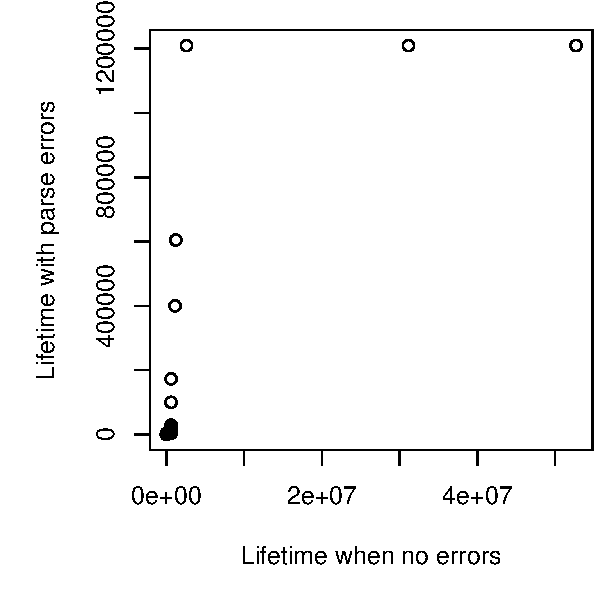
\includegraphics[width=.8\textwidth]{errorsqq.pdf}}
  \caption{A quantile-quantile plot of freshness lifetimes for
    standard compliant headers with and without errors.}
  \label{fig:errorsqq}
\end{figure}



%\bibliographystyle{plain}
\bibliographystyle{abbrv}
%\bibliographystyle{jbact}
%\bibliographystyle{splncs03}
\bibliography{webarch,data,rfc,hypermedia,dynamicity,stat1,specs,vocabs}



\end{document}
